\section{Introduction}
Multi-agent motion planning has been studied extensively in artificial intelligence, robotics and computer games.
The objective is to navigate multiple agents from a set of start positions to corresponding goal positions while avoiding inter-agent collisions as well as collisions with obstacles.
At a broad level, prior approaches can be classified into two categories: decentralized and centralized methods. 
For decentralized algorithms, the planner computes the trajectory for each agent separately for a short time horizon and uses some sort of coordination to avoid intersection between these local trajectories. On the other hand, the centralized methods combine the configuration degrees of each agent into one large high DOF (degree-of-freedom) system, which computes their paths together. Such centralized methods can provide completeness, including resolution-completeness or probabilistic-completeness guarantees. However, they are practical for scenarios with only a few low DOF agents.

\begin{figure}[!ht]
\centering
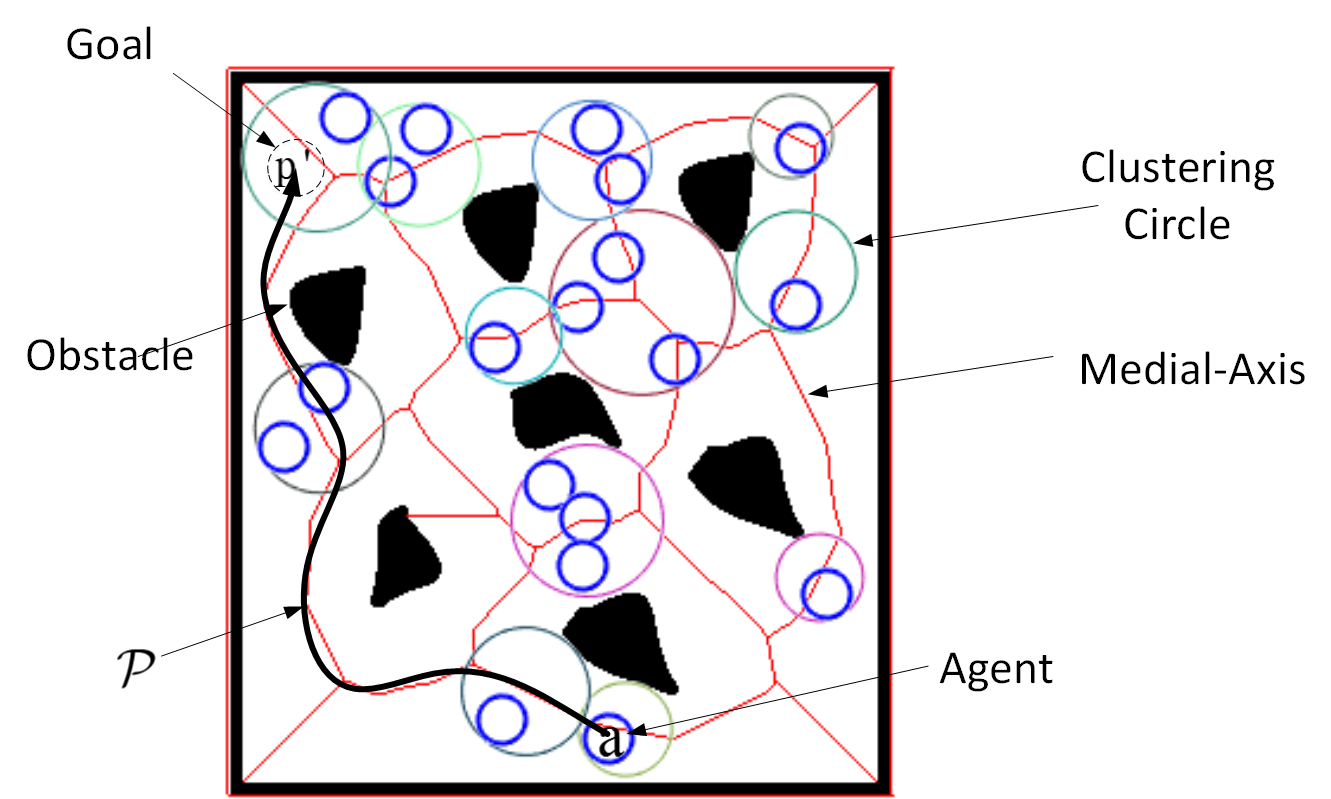
\includegraphics[width=0.8
\linewidth]{figs/Overview.png}
\caption{{\bf Medial Axis based Multi-Agent Planning:} {\em  We provide an overview of our approach. We show the computed path $\mathcal{P}$ for one of the agents moves toward its goal position. Given the black obstacles, we compute the medial axis of the workspace (shown in red) and use that to compute clusters of blue agents. The properties of medial axis are used to design resolution-complete multi-agent planner for arbitrary obstacles. Our approach results in speedups improvement over prior methods.}}
\vspace*{-0.1in}
\label{fig:overview}
\end{figure}
Many previous centralized algorithms are limited to discrete workspaces ~\cite{katsev2013efficient,luna2011push}.
%{\color{red}In discrete workspace motion planning, the agents are homogeneous, that is, they are equal size and does not consider the constraint of dynamic system. On the other hand, 
These methods are limited to homogeneous agents and assume that the workspace is divided into a finite number of discrete units, e.g. uniform grids, and that each agent moves one unit to another in each step. Other planning algorithms have been proposed for a continuous workspace, but they are limited to simple workspaces or assume that the obstacles have piece-wise linear boundaries.  ~\cite{turpin2013goal,krontiris2013feasibility,karamouzas2013space,turpin2013trajectory,turpin2013concurrent}. Furthermore, the running time of these algorithms is governed by the combinatorial complexity of the 2D obstacles, i.e. the number of edges.
%number of obstacles' linear edges. 
%It turns out which can not efficient approximate the obstacles with complex shape. }
In many applications, the agents move in a continuous space and the obstacles in the scene can have arbitrary shapes, including non-convex polygons or curved boundaries. In such scenarios, using a discretization of the continuous workspace into a finite number of units can result in errors or the planner not being able to compute a feasible solution.  

%By taking advantage of this trick, the movements of any agents can be illustrate as inter-cluster and inter-loop moving. 
%It turns out we can deduct if current case exists a solution by checking whether every agent can finish the necessary movements. 

\textbf{Main Results}:
We present a novel and resolution-complete algorithm for multi-agent motion planning problem in a continuous 2D workspace with arbitrarily-shaped obstacles. We make no assumptions about the environment and the obstacles can be represented using piecewise lines or curves. Our approach utilizes the properties of the medial axis of the workspace. In particular, we compute an approximation of the Blum's medial axis using sampling methods. Based on the medial axis, we represent the free-space, i.e. the collision-free subset of the workspace, using a finite set of \textit{elements} connected by \textit{paths}. An element is a subset of free-space that has the same shape as the agent and the path connects two or more elements in the free space. Moreover, we use {\em circle packing} algorithms to represent a group of clustered agents.
Based on this representation and decomposition, we transform the continuous planning problem into a discrete planning problem on graph, with each element being a node and each path being an edge of the graph. 
%The algorithm uses this graph to compute the path for each agent. 
%Based on this formulation, our algorithm can compute a collision-free path for each agent.
%According to these data structures, we design an algorithm and prove it meets minimum spatial requirement to find a solution for this problem.}
%Then we transit  (WHAT DOES TRANSMIT MEAN: NOT A GOOD WORD) each cluster into a discrete unit (WHAT KIND OF DISCRETE UNIT, DEFINE),
% need couple of sentences to explain why cluster can transit to discrete


%Moreover, the computational complexity of our algorithm is not directly irrelevant to the complexity of the environment. 

Our method is able to handle the homogeneous disc-like agents. We prove that our approach is resolution-complete, if an approximate medial-axis of the workspace at any resolution, as well as a solution to the circle packing solution is available. In practice, we sample the boundaries of the obstacles using points and compute the approximate media-axis. In such cases, we show our multi-agent planning algorithm is resolution complete. We have evaluated our algorithm on 2D benchmarks with $40-100$ agents and we highlight the significant improvement in running time (up to $100$X) over prior methods.
%complete if and only if an exactly medial-axis can be extracted from the scene.%without considering the dynamic constraints. 
%The speed of our algorithm mainly depends on the number of agents instead of the shape of obstacles.
%In this paper, our method works on the 2-D workspace but it can be easily extended into 3-D environment. 
